\documentclass[11pt,a4paper]{article}

\usepackage[margin=2.2cm]{geometry}
\usepackage{amsmath,amssymb,amsfonts,amsthm}
\usepackage[T1]{fontenc}
\usepackage{lmodern}
\usepackage{microtype}
\usepackage{enumitem}
\usepackage[hidelinks]{hyperref}
\usepackage{xcolor}
\usepackage{tikz}
\usepackage{listings}
\usepackage{booktabs}
\usetikzlibrary{positioning,arrows.meta,shapes.geometric,fit,calc,decorations.pathreplacing}

\definecolor{matclr}{RGB}{40,103,160}
\definecolor{unitclr}{RGB}{180,70,40}
\definecolor{rawclr}{RGB}{50,140,80}
\definecolor{prodclr}{RGB}{160,60,140}
\definecolor{deadclr}{RGB}{120,120,120}
\definecolor{kept}{RGB}{40,140,80}
\definecolor{cut}{RGB}{170,60,60}

\tikzset{
    mat/.style={circle,draw=matclr,thick,fill=matclr!10,minimum size=8mm,inner sep=1pt},
    raw/.style={mat,draw=rawclr,fill=rawclr!12},
    prod/.style={mat,draw=prodclr,fill=prodclr!12,line width=0.6mm},
    unit/.style={rectangle,draw=unitclr,thick,fill=unitclr!10,minimum height=8mm,minimum width=12mm,rounded corners=1pt,inner sep=2pt},
    edge/.style={-{Stealth[length=2.2mm]},semithick},
    kept/.style={fill=kept!18},
    cut/.style ={fill=cut!18,opacity=0.6},
}

\lstset{
    basicstyle=\ttfamily\small,
    breaklines=true,
    columns=fullflexible,
    keepspaces=true,
    showstringspaces=false,
    xleftmargin=0pt,xrightmargin=0pt,
}

\newcommand{\HyMeKo}{\textsc{HyMeKo}}
\newcommand{\code}[1]{\texttt{\small #1}}
\setlist[itemize]{leftmargin=1.4em,itemsep=2pt,topsep=3pt}

\title{P-graphs in \HyMeKo:\\[2pt]
       \large{\normalfont parse, lower, MSG, SSG, ABB}}
\author{}
\date{2026-05-05}

\begin{document}
\maketitle

\noindent
This brief documents what landed: a P-graph encoding inside the
canonical \HyMeKo{} grammar (idiomatic --- units are
\emph{hyperedges}), an AST $\to$ schema lowering, and Rust
implementations of \emph{Maximal Structure Generation} (MSG),
\emph{Solution Structure Generation} (SSG) and the
\emph{Accelerated Branch-and-Bound} (ABB) of Friedler, Tarj\'an,
Huang and Fan (1992). The pipeline is end-to-end on the worked HDA
example.

\paragraph{The structural choice.} In \HyMeKo, an \code{@}-prefixed
declaration is a hyperedge; without the \code{@} it is a hypernode.
Both carry the same machinery (tags, an optional value, a body of
\code{HyperItem}s) --- the only structural difference is the role
tag carried by \code{@}. This is exactly what a P-graph wants: a
material is a passive resource (hypernode), an operating unit
\emph{is} a hyperedge connecting input materials to output materials.
We thus encode units with \code{@} and put the I/O signature inside
the edge body as a single signed hyperarc.

% ────────────────────────────────────────────────────────────────────
\section{Pipeline}

\begin{center}
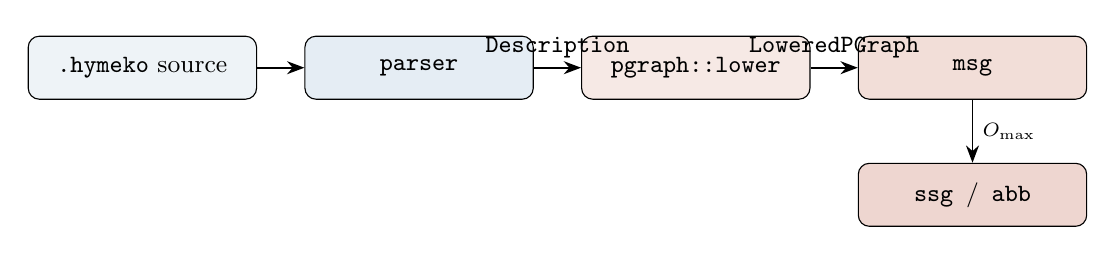
\begin{tikzpicture}[node distance=4.5mm and 6mm, every node/.style={font=\small}]
\node[draw,rounded corners,minimum width=29mm,minimum height=8mm,fill=matclr!8]   (src)  {\code{.hymeko} source};
\node[draw,rounded corners,minimum width=29mm,minimum height=8mm,fill=matclr!12,right=of src] (par)  {\code{parser}};
\node[draw,rounded corners,minimum width=29mm,minimum height=8mm,fill=unitclr!12,right=of par] (low)  {\code{pgraph::lower}};
\node[draw,rounded corners,minimum width=29mm,minimum height=8mm,fill=unitclr!18,right=of low] (msg)  {\code{msg}};
\node[draw,rounded corners,minimum width=29mm,minimum height=8mm,fill=unitclr!22,below=8mm of msg] (alg)  {\code{ssg} \,/\, \code{abb}};

\draw[edge] (src) -- (par);
\draw[edge] (par) -- node[above,font=\scriptsize]{\code{Description}} (low);
\draw[edge] (low) -- node[above,font=\scriptsize]{\code{LoweredPGraph}} (msg);
\draw[edge] (msg) -- node[right,font=\scriptsize]{$O_{\max}$} (alg);
\end{tikzpicture}
\end{center}

% ────────────────────────────────────────────────────────────────────
\section{Encoding a P-graph in the \HyMeKo{} grammar}

A bipartite Material/Operating-Unit graph maps onto the canonical
hypergraph grammar with three conventions:
\begin{itemize}
\item Materials are \emph{hypernodes} tagged \code{<material>}.
\item Operating units are \emph{hyperedges}
  (\code{@}-prefix) tagged \code{<unit>}.
\item Inside a unit body, place exactly one signed hyperarc whose
  signs are the unit's I/O signature: \code{-X} means the unit
  consumes $X$, \code{+X} means it produces $X$.
\end{itemize}
Sub-tags \code{<raw>} and \code{<product>} on materials populate the
raw set $R$ and the demand set $P$. The unit's scalar cost is the
edge's numeric value (read by ABB); a \code{cost N;} child node is
also accepted for back-compat.

\begin{lstlisting}
HDA{}
context {
    Toluene <material, raw>;
    H2      <material, raw>;
    Mix     <material>;
    Benzene <material, product>;
    Methane <material>;

    @Mixer       <unit> 100 { (-Toluene, -H2, +Mix); }
    @Reactor     <unit> 250 { (-Mix, +Benzene, +Methane); }
    @DirectSynth <unit> 800 { (-Toluene, -H2, +Benzene); }
    @Disposal    <unit>  50 { (-Methane); }
}
\end{lstlisting}

\paragraph{Why this is the right encoding.} The grammar's
\code{NodeDecl} and \code{EdgeDecl} are structurally near-identical
--- both accept tags, an optional value, and a body of
\code{HyperItem}s. The \code{@} prefix is purely a role marker, not
a different kind of object. The lowering walks
\code{HyperItem::Node} for materials and \code{HyperItem::Edge} for
units and unifies them into the schema's $(M,O,E_{\mathrm{dir}})$
triple. The signed-incidence semantics built into hyperarcs
($\pm$ for produce/consume) is then exactly what a P-graph needs.

\subsection*{The HDA P-graph}

\begin{center}
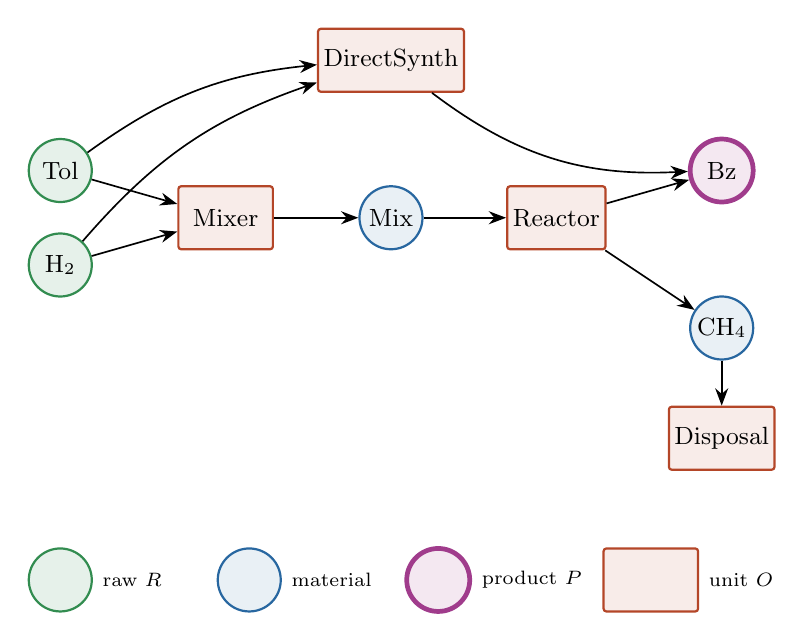
\begin{tikzpicture}[node distance=10mm and 16mm,every node/.style={font=\small}]
% materials (column 1)
\node[raw] (T)   at (0,3.6) {Tol};
\node[raw] (H2)  at (0,2.4) {H$_2$};
\node[mat] (Mix) at (4.2,3) {Mix};
\node[prod](B)   at (8.4,3.6) {Bz};
\node[mat] (Me)  at (8.4,1.6) {CH$_4$};

% units
\node[unit] (Mx) at (2.1,3) {Mixer};
\node[unit] (Rx) at (6.3,3) {Reactor};
\node[unit] (Ds) at (8.4,0.2) {Disposal};
\node[unit] (Dr) at (4.2,5)   {DirectSynth};

% wiring
\draw[edge] (T) -- (Mx);
\draw[edge] (H2) -- (Mx);
\draw[edge] (Mx) -- (Mix);
\draw[edge] (Mix) -- (Rx);
\draw[edge] (Rx) -- (B);
\draw[edge] (Rx) -- (Me);
\draw[edge] (Me) -- (Ds);

\draw[edge,bend left=15] (T) to (Dr);
\draw[edge,bend left=15] (H2) to (Dr);
\draw[edge,bend right=20] (Dr) to (B);

% legend
\begin{scope}[xshift=0cm,yshift=-1.6cm]
\node[raw,label=right:{\scriptsize raw $R$}] at (0,0) {};
\node[mat,label=right:{\scriptsize material}] at (2.4,0) {};
\node[prod,label=right:{\scriptsize product $P$}] at (4.8,0) {};
\node[unit,label=right:{\scriptsize unit $O$}] at (7.5,0) {};
\end{scope}
\end{tikzpicture}
\end{center}

% ────────────────────────────────────────────────────────────────────
\section{AST $\to$ \code{LoweredPGraph}}

\code{hymeko\_pgraph::lower} walks the parsed \code{Description},
descending one level into untagged-node wrappers like
\code{context\{\dots\}}. Tagged \code{HyperItem::Node}s become
materials; tagged \code{HyperItem::Edge}s become units. From each
unit body, a single signed hyperarc is read and converted into one
directed schema edge per signed reference (\code{-X} $\Rightarrow$
$X \to U$, \code{+X} $\Rightarrow$ $U \to X$). The bipartite
invariant is enforced by \code{PGraphSchema::try\_new}; a unit body
using \code{\textasciitilde X} (neutral) is rejected. The lowered
record carries every side-table the algorithms need:
\[
\code{LoweredPGraph} = \big(\text{schema},\, R,\, P,\, M,\, O,\, c,\,
   \text{in}, \text{out}\big),
\]
where $c\colon O \to \mathbb{R}_{\ge 0}$ is the per-unit cost
(default $1.0$).

% ────────────────────────────────────────────────────────────────────
\section{MSG --- Maximal Structure Generation}

The maximal structure $O_{\max}\subseteq O$ is the largest subset
that is both \emph{forward}- and \emph{backward}-feasible. The
implementation iterates two trims to a fixpoint:

\begin{itemize}
\item \textbf{Forward.} Compute the producibility closure
  $C_R(O') = \mathrm{lfp}\,\big[X \mapsto R \cup \{m \mid \exists u
  \in O',\, \mathrm{in}(u) \subseteq X,\, m \in \mathrm{out}(u)\}\big]$.
  Drop every $u\in O'$ whose $\mathrm{in}(u) \not\subseteq C_R(O')$.
\item \textbf{Backward.} Let
  $\mathrm{useful} = P \cup \bigcup_{u\in O'} \mathrm{in}(u)$. Drop
  every $u$ whose $\mathrm{out}(u) \not\subseteq \mathrm{useful}$.
\end{itemize}

Iteration converges in $O(|O|)$ rounds. The backward rule is
``every output is useful,'' \emph{not} ``some output reaches a
product'' --- the latter wrongly drops legitimate consumer / disposal
units (this was today's first MSG bug).

\subsection*{Walk on HDA}

\begin{center}
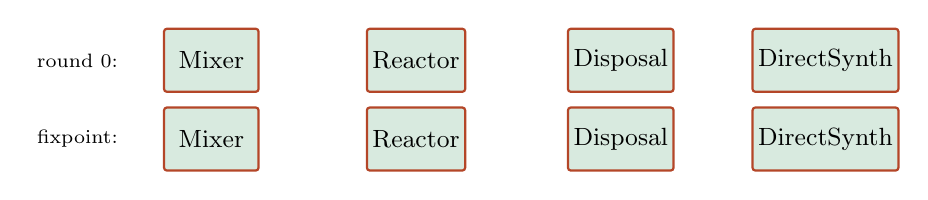
\begin{tikzpicture}[node distance=4mm and 8mm,every node/.style={font=\small}]
\node[unit,kept]  (Mx) at (0,0)   {Mixer};
\node[unit,kept]  (Rx) at (2.6,0) {Reactor};
\node[unit,kept]  (Ds) at (5.2,0) {Disposal};
\node[unit,kept]  (Dr) at (7.8,0) {DirectSynth};
\node[font=\scriptsize] at (-1.7,0) {round 0:};

\node[unit,kept]  (Mx2) at (0,-1.0)   {Mixer};
\node[unit,kept]  (Rx2) at (2.6,-1.0) {Reactor};
\node[unit,kept]  (Ds2) at (5.2,-1.0) {Disposal};
\node[unit,kept]  (Dr2) at (7.8,-1.0) {DirectSynth};
\node[font=\scriptsize] at (-1.7,-1.0) {fixpoint:};
\end{tikzpicture}
\end{center}
On HDA every unit is forward- and backward-feasible, so $O_{\max}=O$.

\subsection*{Walks that prune}

\begin{center}
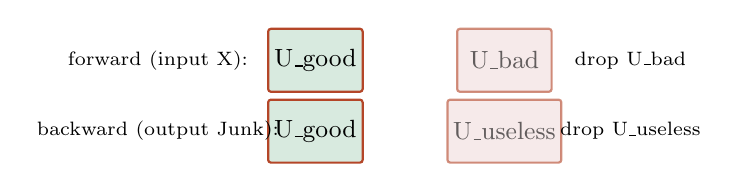
\begin{tikzpicture}[node distance=4mm and 8mm,every node/.style={font=\small}]
% Forward-prune example
\node[unit,kept]  (Ug) at (0,0)   {U\_good};
\node[unit,cut]   (Ub) at (2.4,0) {U\_bad};
\node[font=\scriptsize] at (-2,0) {forward (input X):};
\node[font=\scriptsize] at (4,0) {drop U\_bad};

\node[unit,kept]  (Ug2) at (0,-0.9)   {U\_good};
\node[unit,cut]   (Uu)  at (2.4,-0.9) {U\_useless};
\node[font=\scriptsize] at (-2,-0.9) {backward (output Junk):};
\node[font=\scriptsize] at (4,-0.9) {drop U\_useless};
\end{tikzpicture}
\end{center}

% ────────────────────────────────────────────────────────────────────
\section{SSG --- Solution Structure Generation}

SSG enumerates every $O' \subseteq O_{\max}$ that satisfies:
\begin{enumerate}[label=(\alph*)]
\item \emph{Input consistency:} for every $u\in O'$,
      $\mathrm{in}(u) \subseteq C_R(O')$.
\item \emph{Demand:} every $p \in P$ lies in $C_R(O')$.
\item \emph{No-excess} (strict, default): every produced material
      that is not in $R \cup P$ is consumed by some $u\in O'$.
\end{enumerate}
The implementation enumerates by bitmask over $O_{\max}$ (refuses
silently for $|O_{\max}|>30$, where ABB is the right tool).

On HDA with strict no-excess the feasible set is
\[
\big\{\{\text{Mixer}, \text{Reactor}, \text{Disposal}\},\,
      \{\text{DirectSynth}\}\big\}.
\]
Relaxing (c) admits the by-product-leaving structure
$\{\text{Mixer}, \text{Reactor}\}$ and a few more.

% ────────────────────────────────────────────────────────────────────
\section{ABB --- Accelerated Branch-and-Bound}

ABB performs DFS over the include/exclude lattice of $O_{\max}$ with
two pruning rules:
\begin{itemize}
\item \textbf{Inclusion bound.} Abandon a partial selection whose
  cost has already met or exceeded the current incumbent.
\item \textbf{Reachability bound.} Let
  $\widehat{O} = \mathrm{included} \cup \mathrm{undecided}$. If
  $C_R(\widehat O) \not\supseteq P$, no descendant can be feasible
  --- prune.
\end{itemize}
Branching order is fixed; each step takes ``include'' before
``exclude'', so a feasible incumbent appears early.

\subsection*{ABB tree on HDA (strict)}

\begin{center}
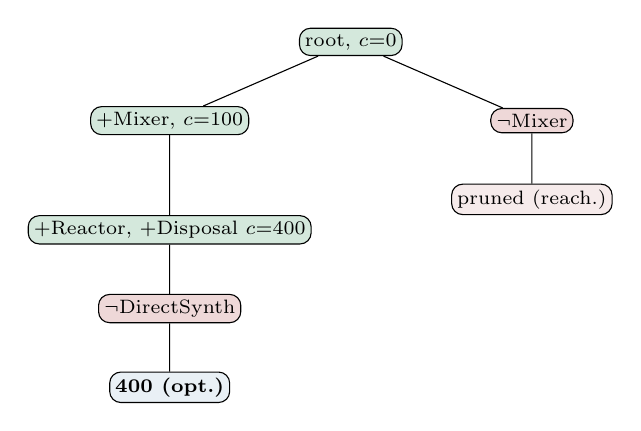
\begin{tikzpicture}[
    level distance=10mm,
    level 1/.style={sibling distance=46mm},
    level 2/.style={sibling distance=10mm},
    every node/.style={font=\scriptsize},
    inc/.style={draw,fill=kept!20,rounded corners,inner sep=2pt},
    exc/.style={draw,fill=cut!20,rounded corners,inner sep=2pt},
    leaf/.style={draw,fill=matclr!10,rounded corners,inner sep=2pt},
    pr/.style={draw,fill=cut!10,rounded corners,inner sep=2pt},
]
\node[inc] {root, $c{=}0$}
  child {node[inc] {$+$Mixer, $c{=}100$}
    child {node[inc,below=2mm] {$+$Reactor, $+$Disposal $c{=}400$}
        child {node[exc] {$\lnot$DirectSynth}
          child {node[leaf] {\textbf{400 (opt.)}}}
        }
    }
  }
  child {node[exc] {$\lnot$Mixer}
    child {node[pr] {pruned (reach.)}}
  };
\end{tikzpicture}
\end{center}
\noindent
Excluding Mixer fails the reachability check (Mix is then
unproducible), so half the tree dies at the second level. The
right-most branch \code{+DirectSynth} is dominated by the inclusion
bound at $c=800>400$.

% ────────────────────────────────────────────────────────────────────
\section{Empirical run on HDA}

\begin{center}
\begin{tabular}{lll}
\toprule
algorithm                      & output                                   & cost \\
\midrule
\textsc{msg}                   & $\{$Mixer, Reactor, Disposal, DirectSynth$\}$ & --- \\
\textsc{ssg} (strict)          & $\{\{$Mx,Rx,Ds$\},\,\{$DS$\}\}$            & --- \\
\textsc{ssg} (relaxed)         & 4 structures incl.\ $\{$Mx,Rx$\}$          & --- \\
\textsc{abb} (strict)          & $\{$Mixer, Reactor, Disposal$\}$           & 400 \\
\textsc{abb} (relaxed)         & $\{$Mixer, Reactor$\}$                     & 350 \\
\bottomrule
\end{tabular}
\end{center}

The pipeline is exercised by \code{hymeko\_pgraph/tests/pgraph\_e2e.rs}
(9 tests, all passing) on top of \code{hymeko\_pgraph}'s 8 schema
unit tests.

% ────────────────────────────────────────────────────────────────────
\section*{What's not done}

A2/A3/A5 axiom checks (\code{axioms.rs}) are still parked --- only
A1 (product membership) and A4 (degree) fire today. SSG above 30
units, multi-optimum reporting in ABB, and reusing
\code{hymeko\_graph}'s cycle enumerator for recycle-loop-aware MSG
remain follow-ups.

\end{document}
